Die bisherigen Szenarien nutzen eine statische Kamera. Das erlaubt zwar konstante Messungen, entspricht allerdings keiner realistischen Situation. Normalerweise wird die Kamera bewegt und rotiert. Die folgenden Szenarien stellen dynamische Situationen dar, in denen die Kamera bewegt wird. In diesem Szenario wird die Kamera dauerhaft rotiert mit einer Winkelgeschwindigkeit von \SI{45}{\degree\per\second}. Eine Reihe von Bildschirmfotos, die die Rotation zeigt, ist in Abbildung~\ref{fig:rotate} zu sehen.
\begin{figure}
	\centering
	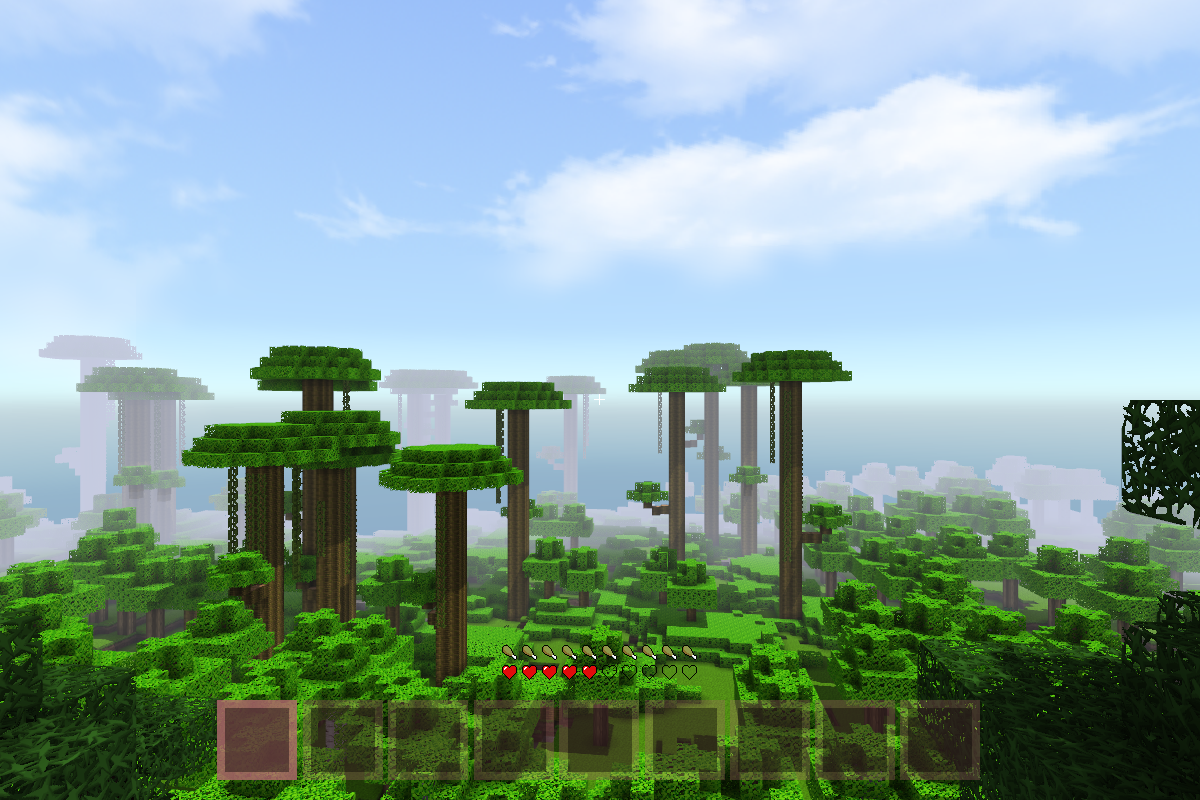
\includegraphics[width=.32\textwidth]{rotate-1.png}
	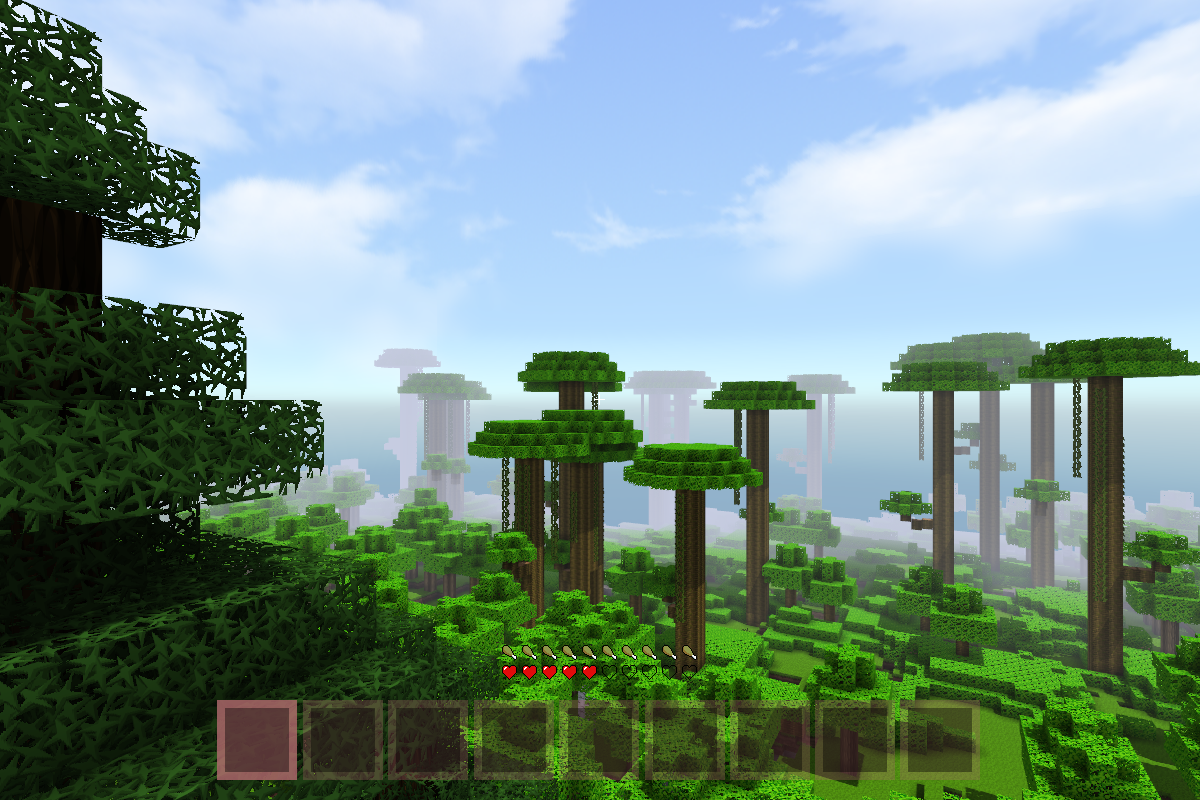
\includegraphics[width=.32\textwidth]{rotate-2.png}
	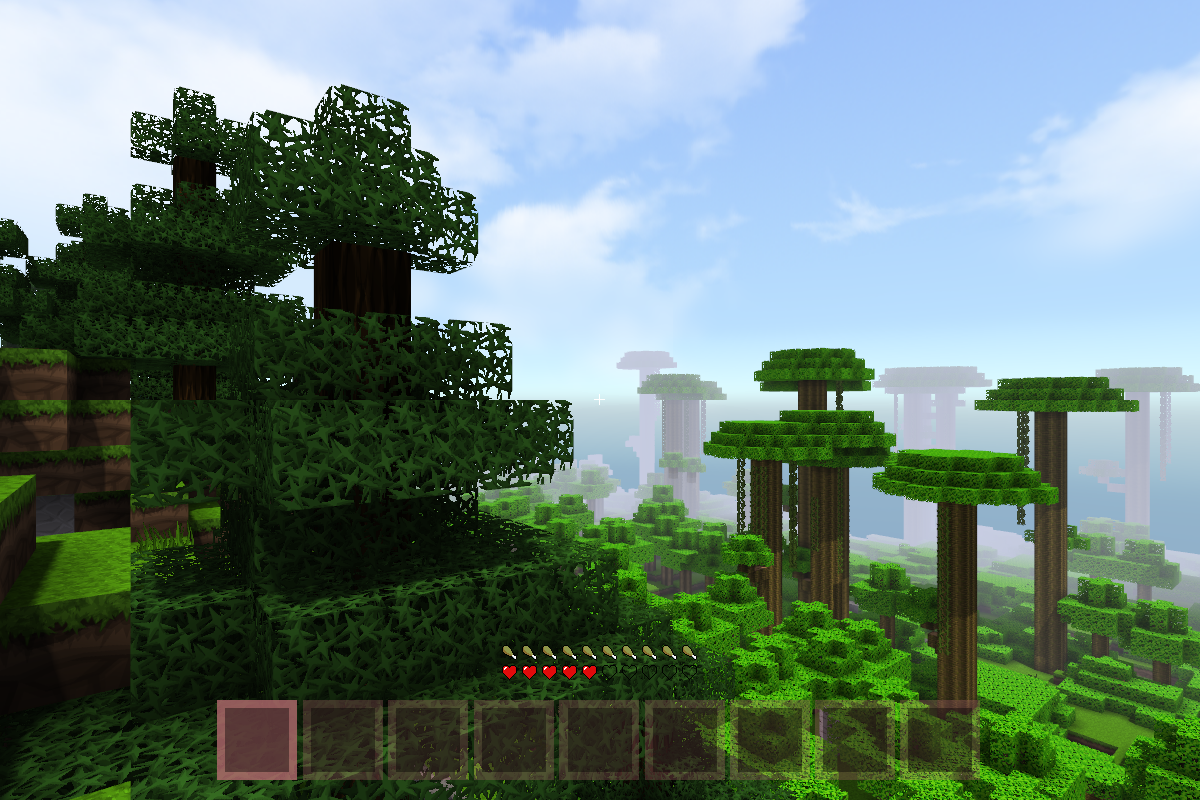
\includegraphics[width=.32\textwidth]{rotate-3.png}\\[4pt]
	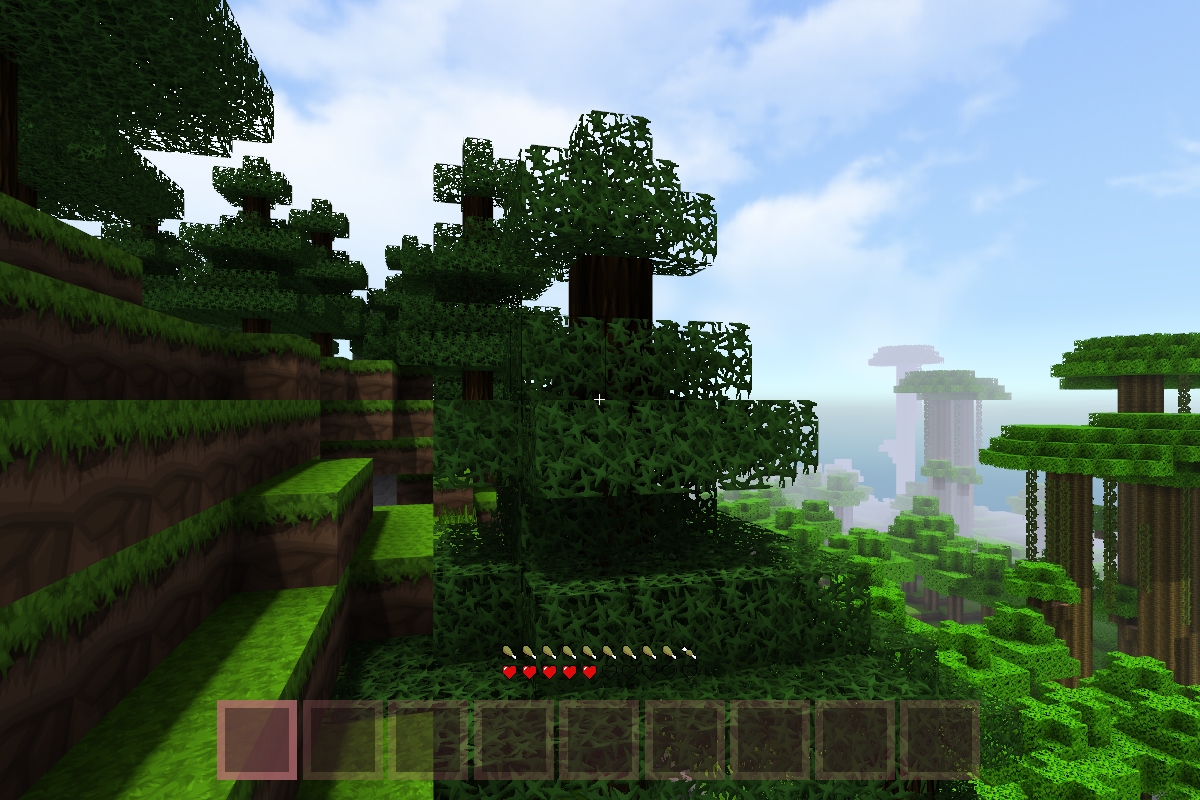
\includegraphics[width=.32\textwidth]{rotate-4.png}
	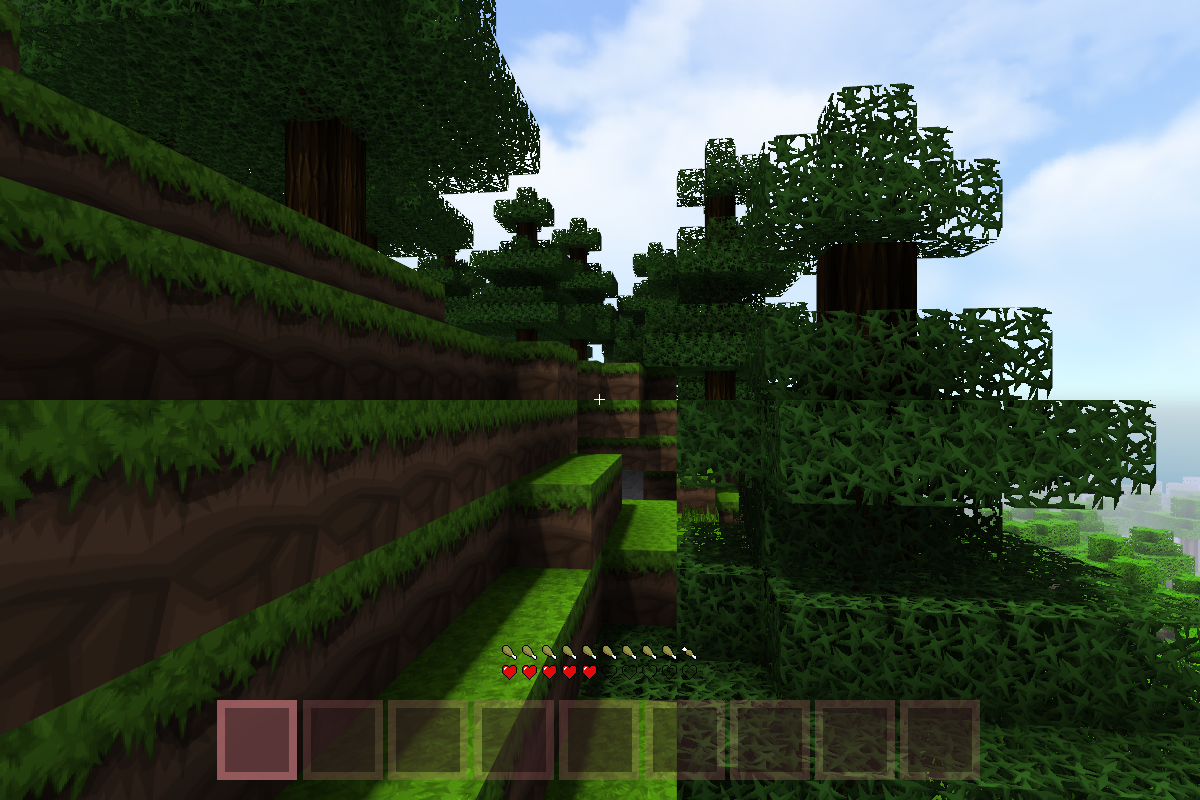
\includegraphics[width=.32\textwidth]{rotate-5.png}
	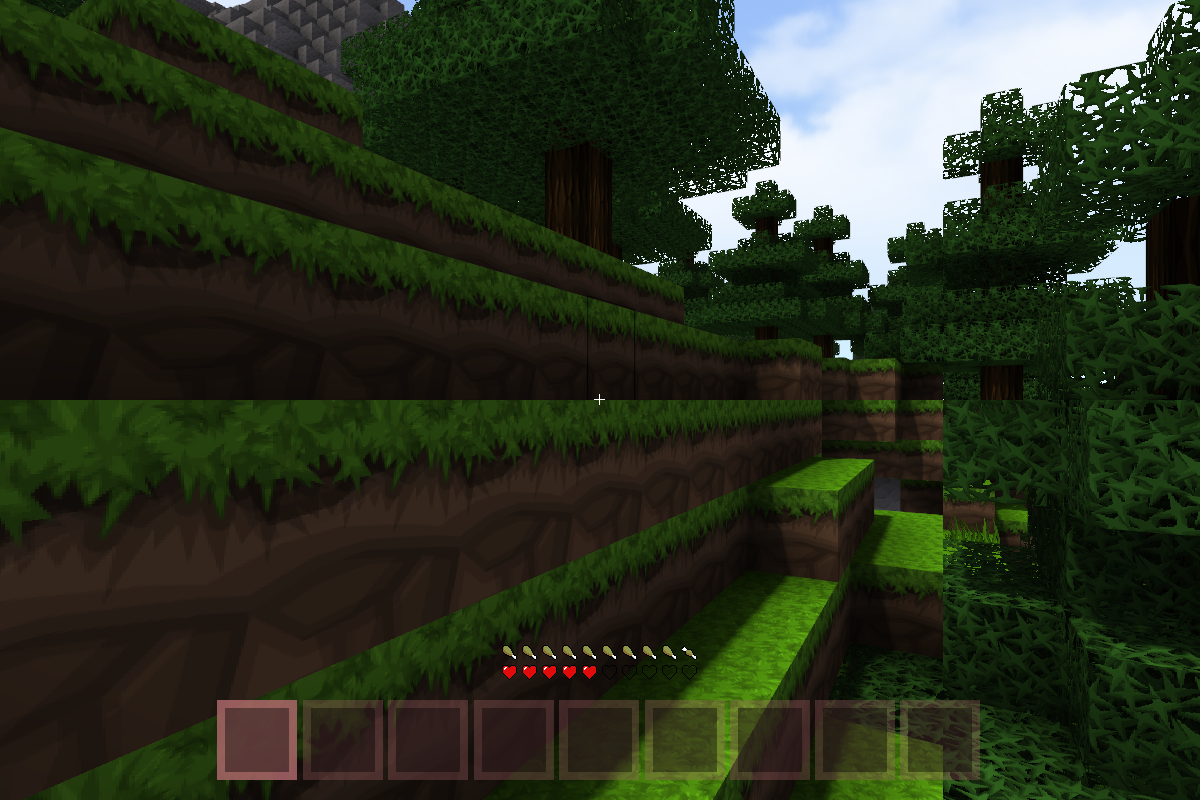
\includegraphics[width=.32\textwidth]{rotate-6.png}
	%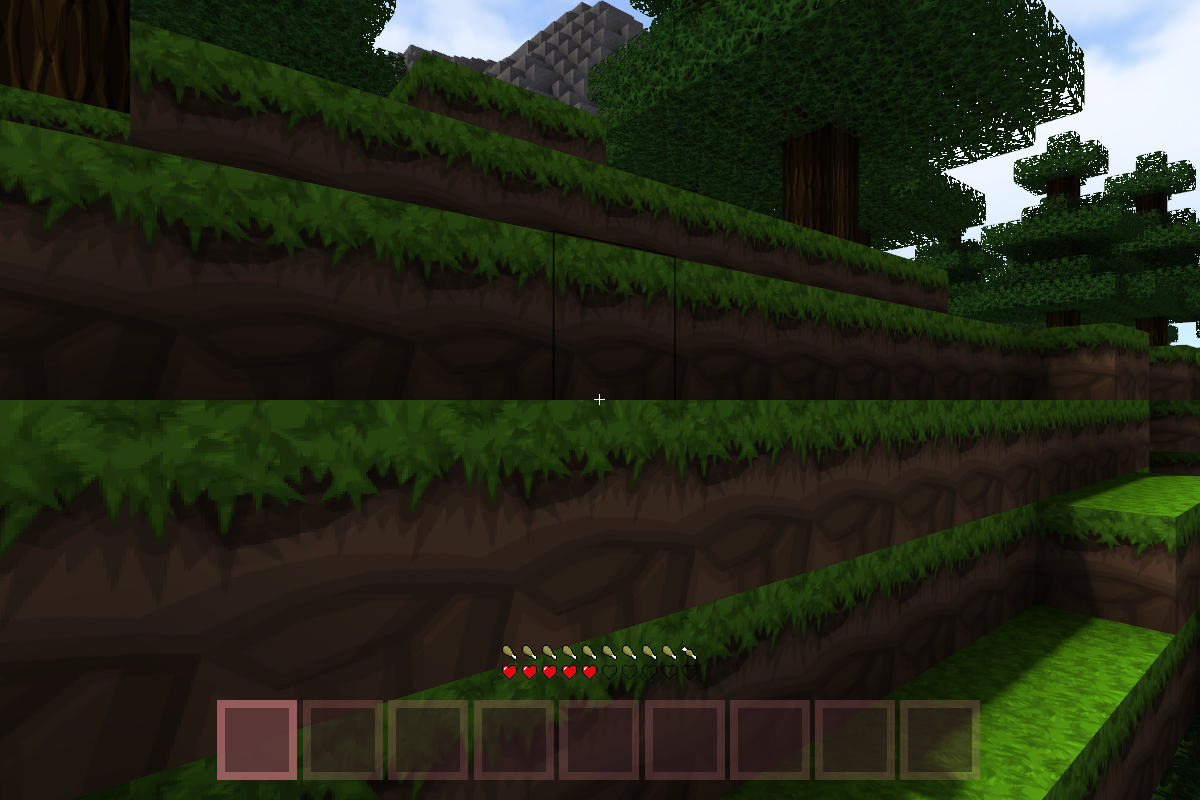
\includegraphics[width=.24\textwidth]{rotate-7.png}
	%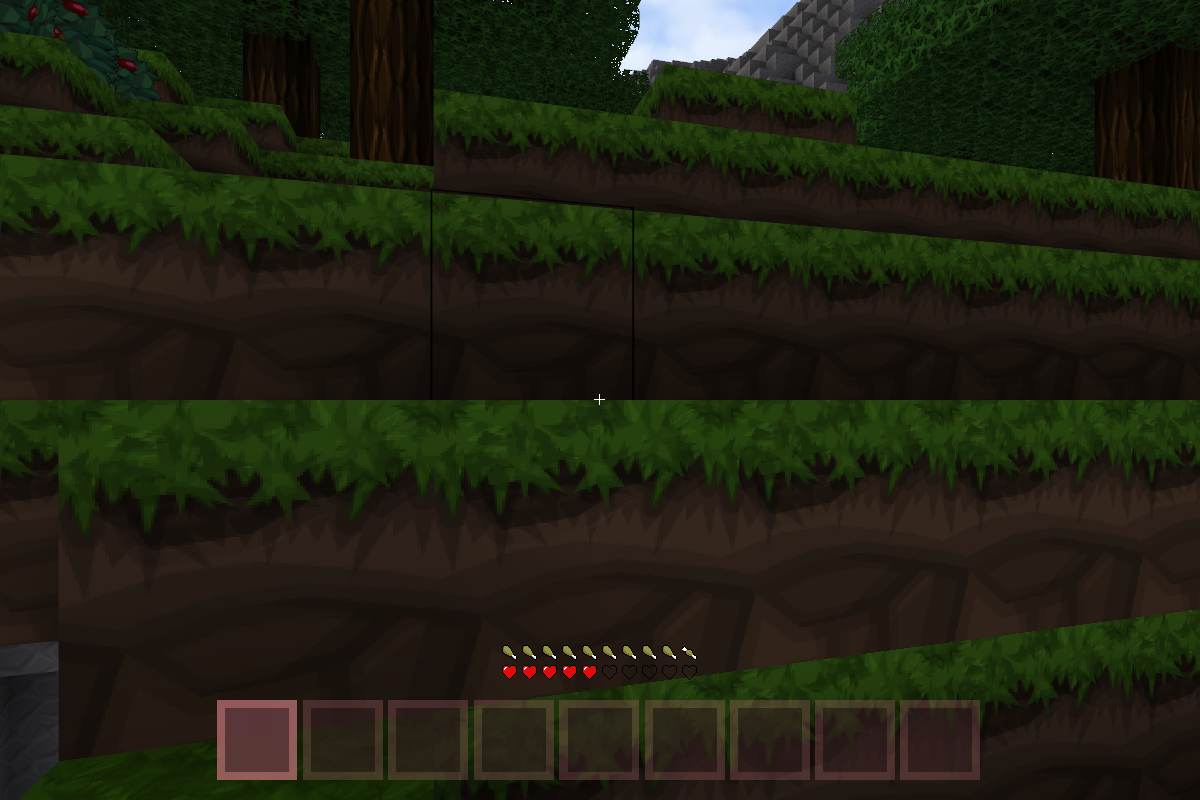
\includegraphics[width=.24\textwidth]{rotate-8.png}
	\caption{Reihe von Bildschirmfotos, die die Rotation in Szenario 4 zeigt. Die Rotationsrichtung ist gegen den Uhrzeigersinn. Die Bildschirmfotos wurden in einem Zeitabstand von \SI{500}{\milli\second} aufgenommen.}\label{fig:rotate}
\end{figure}
Wie an den Bildschirmfotos zu erkennen ist, wird auch für dieses Szenario der Seed 0 genutzt.

\paragraph{\ac{fps}}
Betrachtet man den Verlauf der \ac{fps} in diesem Szenario, ergibt sich ein zu den vorherigen Szenarien deutlich abweichendes Muster. Dies ist in Abbildung in Abbildung~\ref{fig:seed-0-rotate-fps} zu sehen.
\begin{figure}[!htbp]
	\fpsplot{seed-0-rotate}
	\caption{Graph des Verlaufs der Framerate in Szenario 4: Welt-Rotation.}\label{fig:seed-0-rotate-fps}
\end{figure}
\sysB{} beginnt 5 Sekunden später mit der Erzeugung von Bildern als \sysA{}. Zwar stimmt diese Beobachtung mit denen der anderen Szenarien überein, aber das Verhalten der Framerate in der Hauptphase ist verglichen mit den anderen Szenarien einzigartig. In \sysA{} und in \sysB{} noch deutlicher sind zyklische Schwankungen der \ac{fps} zu erkennen. Die Periode der Schwankungen beträgt in beiden Systemen 8 Sekunden. Das entspricht exakt der Periode der Rotation ($8\cdot \SI{45}{\degree} = \SI{360}{\degree}$). Unter Betrachtung der Bildschirmfotos in Abbildung~\ref{fig:rotate} lässt sich eine Hypothese aufstellen, woher diese Schwankungen kommen. In Seed 0 startet der Spielercharakter in der Nähe eines Berges. Ist die Kamera dem Tal zugewandt, müssen deutlich mehr Elemente gezeichnet werden, als wenn die Kamera dem Berg zugewandt ist. Durch die Rotation ändert sich also die Arbeitslast für die \ac{gpu} periodisch.

Durchschnittlich steigt die Bildwiederholrate von \SI{134}{\fps} in \sysA{} auf \SI{378}{\fps} in \sysB{}. Das ist eine Steigerung von \SI{182}{\percent}. In beiden Systemen ist die Framerate geringer als im Szenario Welt-Statisch. Der Anstieg der Framerate von \sysA{} zu \sysB{} ist allerdings höher. \sysA{} erreicht ein Maximum von \SI{152}{\fps} und ein Minimum von \SI{113}{\fps}, was einen Unterschied von \SI{39}{\fps} darstellt. \sysB{} erreicht maximal \SI{474}{\fps} und sinkt auf bis zu \SI{287}{\fps}, das ist eine Schwankung von \SI{187}{\fps}.

\paragraph{\ac{cpu}}
Im Gegensatz zu der Bildwiederholrate ist in der Auslastung der \ac{cpu} beinahe keine Schwankung zu erkennen. Insbesondere ist keine Periode von 8 Sekunden zu erkennen, wie Abbildung~\ref{fig:seed-0-rotate-cpu} erkennen lässt.
\begin{figure}[!htbp]
	\cpuplot{seed-0-rotate}
	\caption[Graph des Verlaufs der \glsentryshort{cpu}-Auslastung in Szenario 4: Welt-Rotation.]{Graph des Verlaufs der \ac{cpu}-Auslastung in Szenario 3: Welt-Statisch.}\label{fig:seed-0-rotate-cpu}
\end{figure}
Tatsächlich ist der Graph \ac{cpu}-Last beinahe nicht von dem in Szenario 3 zu unterscheiden, mit der Ausnahme der Startphase. Hier sinkt die Auslastung der \ac{cpu} zum ersten Mal in \sysB{} früher als in \sysA{}. Die durchschnittliche Last der Systeme  ist mit \SI{13}{\percent} in \sysA{} und \SI{23}{\percent} in \sysB{} allerdings identisch zum Welt-Statisch Szenario.

Die Tatsache, dass die Auslastungsmessung in \sysB{} zwei Sekunden früher endet als in \sysA{}, ist ein Indiz dafür, dass die Messungen aus einem unbekannten Grund zeitlich verschoben sind. Das würde auch erklären, warum die Startphase in der \ac{cpu}-Auslastung zum ersten Mal in \sysB{} schneller endet als in \sysA{}. Zusätzlich ist die Startphase in der Messung der \ac{fps} in Gegensatz dazu weiterhin mit den vorherigen Szenarien konsistent. 

\paragraph{\ac{gpu}}
Auch der Auslastungsgraph der \ac{gpu} (siehe Abbildung~\ref{fig:seed-0-rotate-gpu}) unterstützt die Hypothese, dass die Startphase in der \ac{cpu}-Last in diesem Szenario aufgrund eines Messfehlers in \sysA{} länger als in \sysB{} ist. Abbildung~\ref{fig:seed-0-rotate-gpu} ist wieder eine längere Startphase von einigen Sekunden in \sysB{} zu erkennen. Durchschnittlich liegt die Auslastung der \ac{gpu} in \sysA{} bei \SI{37}{\percent} und in \sysB{} bei \SI{53}{\percent}. 

Weiter lässt sich die Aussage scheinbar festigen, dass die Schwankungen der Framerate mit der Last der \ac{gpu} zusammenhängen. Auch hier lässt sich eine periodische Schwankung von 8 Sekunden erkennen. 
\begin{figure}[!htbp]
	\gpuplot{seed-0-rotate}
	\caption[Graph des Verlaufs der \glsentryshort{gpu}-Auslastung in Szenario 4: Welt-Rotation.]{Graph des Verlaufs der \ac{gpu}-Auslastung in Szenario 3: Welt-Statisch. Aufgrund der unterschiedlich langen Startphasen ist Schwankung Last in den Systemen zeitlich verschoben.}\label{fig:seed-0-rotate-gpu}
\end{figure}
Die Tatsache, dass diese Schwankung in \sysA{} wie bei der Framerate kleiner ist, als in \sysB{}, führt allerdings zu einer anderen Vermutung. Es ist möglich, dass die Framerate und die \ac{gpu}-Last jeweils von der Belastung des Simulations-Threads abhängen. Die \ac{cpu} des Testsystems besitzt acht Hardware-Threads. Die Last der \ac{cpu} liegt in allen bisherigen Szenarien in \sysA{} bei \SI{13}{\percent} was in etwa $\frac{1}{8} = \SI{12,5}{\percent}$ der Maximallast entspricht. Dieser Wert lässt sich so interpretieren, dass einer der acht Hardware-Threads vollständig ausgelastet ist. Das legt zusammen mit der Tatsache, dass die Last der \ac{gpu} immer unter \SI{100}{\percent} liegt, einen \ac{cpu}-Flaschenhals bezogen auf die Leistung nahe. Diese These wird weiter dadurch unterstützt, dass die Verläufe von \ac{fps} und \ac{gpu}-Auslastung deckungsgleich und nicht gegengleich sind. Wäre die höhere Last der \ac{gpu} für eine geringere Bildwiederholrate verantwortlich, würde man ein gegenläufiges Verhalten erwarten. Außerdem würde diese Vermutung auch erklären, warum die Schwankung der Bildwiederholrate in \sysB{} höher als in \sysA{} ist, denn durch die nebenläufige Architektur kann die Leistung des einen Hardware-Threads vollkommen für die Berechnung der Simulation genutzt werden und muss nicht auf Simulation und Rendering aufgeteilt werden.

Diese Vermutungen ließen sich weiter untersuchen, indem die Auslastung der einzelnen Hardware-Threads gemessen wird. Die nötigen Messungen lassen sich im Rahmen dieser Arbeit aber nicht mehr durchführen. 

\paragraph{\ac{ram}}
Die Nutzung des Hauptspeichers, zu sehen in Abbildung~\ref{fig:seed-0-rotate-mem}, entwickelt sich in Szenario Welt-Rotation anders als in Szenario Welt-Statisch.
\begin{figure}[!htbp]
	\memplot[xticklabels={,,},xlabel={}]{seed-0-rotate-multi-mem.csv}{\sysA{}}
	\\\memplot{seed-0-rotate-multi-mem.csv}{\sysB{}}
	\caption{Graph des Verlaufs der Speichernutzung in Szenario 4: Welt-Rotation.}\label{fig:seed-0-rotate-mem}	
\end{figure} 
\sysA{} nutzt mit durchschnittlich \SI{1267}{\mega\byte} etwas mehr Speicher als im letzten Szenario, \sysB{} mit \SI{1441}{\mega\byte} statt \SI{1793}{\mega\byte} weniger als zuvor. Somit ergibt sich in diesem Szenario ein Anstieg von \SI{14}{\percent} statt \SI{44}{\percent}. 

Derselbe Trend lässt sich im kurzweiligen Verbrauch von Speicher erkennen. \sysA{} hat einen Verbrauch von durchschnittlich \SI{101}{\mega\byte\per\second} und \sysB{} nutzt \SI{187}{\mega\byte\per\second}, was einen Anstieg von \SI{85}{\percent} durch den Wechsel von \sysA{} zu \sysB{} bedeutet.
